\documentclass[12pt]{article}
\usepackage[spanish,mexico]{babel}
	\selectlanguage{spanish}
\usepackage{graphicx}
\usepackage{amsmath}
\usepackage{wrapfig}
\usepackage{float}
\usepackage[utf8]{inputenc}


\title{Actividad 1: Preparando documentos científicos con \LaTeX}
\author{Ana Gabriela Carretas Talamante}
\date{22 de enero de 2016}

\begin{document}
\maketitle
\section{Introducción}
Las matemáticas de los péndulos son generalmente complicadas. Se pueden asumir suposiciones simplificadas, entrando entonces en el caso del péndulo simple. De esta forma las ecuaciones de movimiento pueden ser resueltas analíticamente para oscilaciones con amplitudes pequeñas.
\section{Péndulo de gravedad simple}
Un péndulo simple es el modelo ideal de un péndulo real. Contempla las siguientes suposiciones:
\begin{itemize}
\item La cuerda con la que oscila el péndulo tiene una masa despreciable, es rígida y siempre se mantiene tensa.
\item El péndulo se maneja como masa puntual.
\item El movimiento se realiza en dos dimensiones, i.e., traza un arco al moverse.
\item El movimiento no pierde energía por la resistencia del aire o la fricción.
\item El campo gravitacional es uniforme.
\item El soporte que detiene al sistema no se mueve.
\end{itemize}
La ecuación diferencial que representa el movimiento de un péndulo simple es:
\begin{equation}
\label{1}
\frac{d^2\theta}{dt^2} + \frac{g}{l}\sin\theta=0
\end{equation}
donde $g$ es la aceleración causada por la gravedad, $l$ es la longitud del péndulo y $\theta$ es el desplazamiento angular.
Esta ecuación puede obtenerse de tres maneras diferentes, presentadas a continuación.

\subsection{A partir de la ``Fuerza"}
\begin{wrapfigure}{r}{0.4\textwidth}
\begin{center}
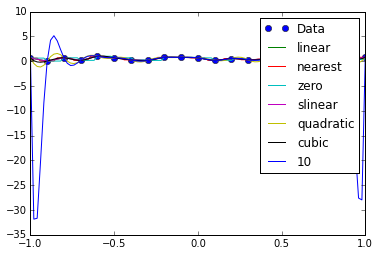
\includegraphics[width=0.35\textwidth]{1.png}
\end{center}
\caption{Diagrama de fuerzas de un péndulo simple \cite{1}.}
\end{wrapfigure}
Podemos observar las fuerzas que actúan sobre un péndulo simple prestando atención a la figura 1. El ángulo $\theta$ es medido en radianes; la flecha azul es la fuerza gravitacional y las rosadas sus componentes. La dirección de la velocidad instantánea del péndulo está señalada con la línea roja, siempre tangente al círculo verde donde realiza el movimiento mismo. \\\\
Teniendo en cuenta la Segunda Ley de Newton, $F=ma$, nos fijamos en el eje tangencial pues es el que realiza el movimiento del péndulo. Entonces:
\begin{alignat}{2}
F=-mg\sin\theta=ma \\
a=-g\sin\theta
\end{alignat}
La aceleración linear $a$ sobre le eje rojo puede relacionarse con el cambio en $\theta$ por las fórmulas de longitud de arco. Sea $s$ la longitud del arco:
\begin{alignat}{3}
s&=l\theta \\
v&=\frac{ds}{dt}=l\frac{d\theta}{dt} \\
a&=\frac{d^2s}{dt^2}=l\frac{d^2\theta}{dt^2}
\end{alignat}
Así, llegamos a \eqref{1},
\begin{alignat}{2}
l\frac{d^2\theta}{dt^2}=-g\sin\theta \\
\frac{d^2\theta}{dt^2}+\frac{g}{l}\sin\theta=0.
\end{alignat}

\subsection{A partir de la ``Torca"}
Definimos la torca del péndulo usando a la fuerza ejercida por la gravedad.
\begin{alignat}{1}
\tau = l \times F_g
\end{alignat}
Ahora solo se considerará la magnitud de la torca del péndulo:
\begin{alignat}{1}
|\tau|=-mgl\sin\theta
\end{alignat}
Reescribimos su momento angular y consideramos solo su magnitud y su derivada con respecto al tiempo:
\begin{alignat}{2}
|L|=mr^2\omega&=ml^2\frac{d\theta}{dt}\\
\frac{d}{dt}|L|&=ml^2\frac{d^2\theta}{dt^2}
\end{alignat}
Como $\displaystyle \tau=r\times F=\frac{dL}{dt}$, podemos igualar las magnitudes de la torca y el momento angular, obteniendo \eqref{1}:
\begin{alignat}{2}
-mgl\sin\theta=ml^2\frac{d^2\theta}{dt^2} \\
\frac{d^2\theta}{dt^2} + \frac{g}{l}\sin\theta=0 
\end{alignat}

\subsection{A partir de la ``Energía"}
\begin{figure}[H]
\centering
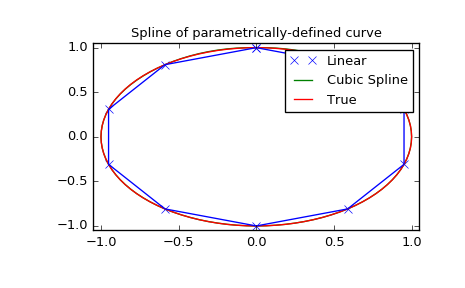
\includegraphics[width=7cm]{2.png}
\caption{Trigonometría de un péndulo simple \cite{2}.}
\end{figure}
La ecuación \eqref{1} también puede obtenerse por medio del principio de conservación de energía; este indica que la energía potencial gravitacional se transforma en energía cinética. Como en el sistema no se pierde energía, los cambios de energía se igualan:
\begin{equation}
\frac{1}{2}mv^2=mgh
\end{equation}
Escribimos la velocidad en términos de $\displaystyle\frac{d\theta}{dt}$:
\begin{alignat}{2}
v=l\frac{d\theta}{dt}&=\sqrt{2gh} \\
\frac{d\theta}{dt}&=\frac{1}{l}\sqrt{2gh}
\end{alignat}
Como se muestra en la figura 2, podemos escribir a $h$ en términos de $\theta$ y $\theta_0$. Sustituyendo en (17):
\begin{equation}
\label{2}
\frac{d\theta}{dt}=\sqrt{\frac{2g}{l}(\cos\theta-\cos\theta_0)}
\end{equation}

Esta ecuación es conocida como la primera integral del movimiento, pues da la velocidad en términos de la posición e incluye una constante de integración relacionada con el desplazamiento inicial. Derivando dos veces con respecto al tiempo para obtener la aceleración, llegamos a \eqref{1}.

\section{Aproximación para amplitudes pequeñas}
La ecuación diferencial que describe el movimiento del péndulo simple no se resuelve sencillamente, y no hay solución analítica para ella. Pero si se añade una restricción en la amplitud de oscilación, resulta una forma de donde es fácil de obtener una solución. Si asumimos que $\theta \ll 1$, entonces $\sin\theta\approx\theta$, obteniendo así la ecuación del oscilador armónico:
\begin{equation}
\frac{d^2}{dt^2}+\frac{g}{l}\theta=0
\end{equation}
Si resolvemos con las siguientes condiciones iniciales, $\theta(0)=\theta_0, \frac{d\theta}{dt}(0)=0$:
\begin{equation}
\theta(t)=\theta_0\cos\left(\sqrt{\frac{g}{l}}t\right) \qquad \theta_0\ll1
\end{equation}
Este resulta en un movimiento armónico simple. El período del movimiento es:
\begin{equation}
T_0=2\pi\sqrt{\frac{l}{g}}\qquad \theta_0\ll1
\end{equation}
también conocido como la Ley del período de Christiaan Huygens.

\subsection{Regla del pulgar para la medida del péndulo}
La expresión (21) también se puede escribir como $l=\frac{g}{\pi ^2}\times\frac{T_0 ^2}{4}$. En el SI, tomando la medicioón sobre la superficie de la Tierra, el valor de $\frac{g}{\pi ^2}\approx1$. Así, una aproximación relativamente aceptable para la longitud y el período son:
\begin{alignat}{2}
l&\approx \frac{T_0 ^2}{4} \\
T_0&\approx 2\sqrt{l}
\end{alignat}
donde $T_0$ es el número de segundos que tarda en dar una oscilación y $l$ es medida en metros.

\section{Período de amplitud arbitraria}
Para amplitudes que superan la designada con la aproximación para amplitudes pequeñas, uno puede calcular el período exacto si primero inviertes la ecuación para la velocidad angular \eqref{2}, y luego para mayor practicidad, integrando 4 veces un cuarto de ciclo:
\begin{alignat}{3}
&\frac{dt}{d\theta}=\sqrt{\frac{l}{2g}}\frac{1}{\sqrt{\cos\theta-\cos\theta_0}} \\
&T=4t(\theta_0\to0)\\
&T=4\sqrt{\frac{l}{2g}}\int_{0}^{\theta_0} \frac{1}{\sqrt{\cos\theta-\cos\theta_0}}d\theta
\end{alignat}
Esta integral también se puede escribir en términos de integrales elípticas como
\begin{equation}
T=4\sqrt{\frac{l}{g}}F\left(\frac{\theta_0}{2},\csc{\frac{\theta_0}{2}}\right) \csc{\frac{\theta_0}{2}}
\end{equation}
Donde $F$ es la integral elíptica incompleta de primera especie definida por
\begin{equation}
F(\varphi,k)=\int_0^\varphi \frac{1}{\sqrt{1-k^2\sin^2u}} du
\end{equation}
O más conscisamente, haciendo la sustitución $\displaystyle\sin u = \frac{\sin{\frac{\theta}{2}}}{\sin{\frac{\theta}{2}}}$ expresando a $\theta$ en términos de $u$,
\begin{equation}\label{3}
T=4\sqrt{\frac{l}{g}}K\left(\sin^2\left(\frac{\theta_0}{2}\right)\right)
\end{equation}
Donde $K$ es la integral elíptica completa de primera especie definida por
\begin{equation}
K(k)=F\left(\frac{\pi}{2},k\right)=\int_{0}^{\frac{\pi}{2}} \frac{1}{\sqrt{1-k^2\sin^2u}} du
\end{equation}
La ecuación \eqref{3} se puede solucionar con distintos métodos, presentados a continuación.

\subsection{Solución polinómica de Legendre para la integral elíptica}
En base a la ecuación \eqref{3} y la solución polinómica de Legendre para la integral elíptica:
\begin{equation*}
K(k)=\frac{\pi}{2}\left\{1+\left(\frac{1}{2}\right)^2k^2+\left(\frac{1\cdot3}{2\cdot4}\right)^2k^4+\cdots+\left[\frac{(2n-1)!!}{(2n)!!}\right]^2k^{2n}+\cdots\right\}
\end{equation*}
Donde $n!!$ denota el doble factorial, una solución exacta para el período de un péndulo es:
\begin{align*}
T&=2\pi\sqrt{\frac{l}{g}}\Bigg(1+\left(\frac{1}{2}\right)^2\sin^2\left(\frac{\theta_0}{2}\right)+\left(\frac{1\cdot3}{2\cdot4}\right)^2\sin^4\left(\frac{\theta_0}{2}\right)+\left(\frac{1\cdot3\cdot5}{2\cdot4\cdot6}\right)^2\sin^6\left(\frac{\theta_0}{2}\right)+\cdots\Bigg) \\
&=2\pi\sqrt{\frac{l}{g}}\cdot\sum_{n=0}^{\infty}\left[\left(\frac{(2n)!}{(2^n\cdot n!)^2}\right)^2\cdot\sin^{2n}\left(\frac{\theta_0}{2}\right)\right]
\end{align*}
En la figura 3, $T_0$ representa la aproximación lineal, y de $T_2$ a $T_{10}$ se incluyen respectivamente los términos hasta la segunda o décima potencia.

\begin{figure}[H]
\centering
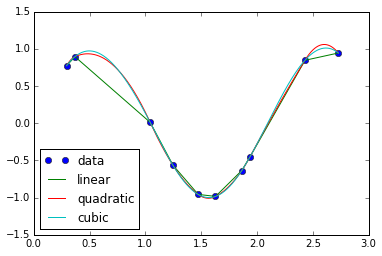
\includegraphics[width=7cm]{3.png}
\caption{Errores relativos unsando la serie de potencias \cite{3}.}
\end{figure}


\subsection{Solución en serie de potencias para la integral elíptica}
Otra formulación pra la solución puede encontrarse en la siguiente serie de Maclaurin:
\begin{equation} \label{4}
\sin{\frac{\theta_0}{2}}=\frac{1}{2}\theta_0-\frac{1}{48}\theta_0^3+\frac{1}{3840}\theta_0^5-\frac{1}{645120}\theta_0^7+\cdots
\end{equation}
\eqref{4} es utilizada en la solución polinómmica de Legendre. La serie de potencias resultante es \cite{4}:
\begin{equation}
T=2\pi\sqrt{\frac{l}{g}}\left(1+\frac{1}{16}\theta_0^2+\frac{11}{3072}\theta_0^4+\frac{173}{737280}\theta_0^6+\frac{22931}{1321205760}\theta_0^8+\cdots\right)
\end{equation}


\subsection{Solución con la media aritmética-geométrica para la integral elíptica}

De \eqref{3} y la solución con la media aritmética-geométrica para la integral elíptica:
\begin{equation}
K(k))=\frac{\frac{\pi}{2}}{M(1-k,1+k)}
\end{equation}
donde $M(x,y)$ es la media aritmética-geométrica de $x$ y $y$. Esto produce una fórmula alternativa y que converge rápidamente para el período \cite{5}:
\begin{equation}
T=\frac{2\pi}{M(1,\cos{\frac{\pi}{2}})}\sqrt{\frac{l}{g}}
\end{equation}

\pagebreak

\begin{thebibliography}{6}

\bibitem{1}
Krishnavedala (2013),
\emph{A simple pendulum in gravity and the forces acting on it}. Recuperado el 19 de enero de 2016 de https://upload.wikimedia.org/wikipedia/commons/6/66/Pendulum\_gravity.svg 

\bibitem{2}
Krishnavedala (2012),
\emph{Simple pendulum}. Recuperado el 19 de enero de 2016 de https://upload.wikimedia.org/wikipedia/commons/1/11/Simple\_pendulum\_height.svg 

\bibitem{3}
Ferreire, R. (2007),
\emph{Pendulum Relative Error 90a}. Recuperado el 19 de enero de 2016 de https://upload.wikimedia.org/wikipedia/en/6/60/Pendulum\_Rel\_Error90a.png 

\bibitem{4}
Nelson, R; Olsson, M. G. (1986),
\emph{The pendulum-Rich physics from a simple system}.
American Journal of Physics,
54 (2).

\bibitem{5}
Carvalhaes, C.; Suppes, P. (2008), \emph{Approximations for the period of the simple pendulum based on the arithmetic-geometric mean}. 
American Journal of Physics,
76 (12).

\bibitem{6}
Wikipedia.
\emph{Pendulum (mathematics)}.
Recuperado el 22 de enero de 2016 de https://en.wikipedia.org/wiki/Pendulum\_(mathematics)
\end{thebibliography}

\end{document}

